%%%%%%%%%%%%%%%%%%%%%%%%%%%%%%%%%%%%%%%%%%%%%%%%%%%%%%%%%%%%%%%%
% %
% Seth Cram %
% ECE351 Section 53 %
% Lab 11 %
% Due 04/12/2022 %
% Any other necessary information needed to navigate the file %
%
%
% %
%%%%%%%%%%%%%%%%%%%%%%%%%%%%%%%%%%%%%%%%%%%%%%%%%%%%%%%%%%%%%%%%
%%%%%%%%%%%%%%%%%%%%%%%%%%%%%%%%%%%%%%%%%%%
%%% DOCUMENT PREAMBLE %%%
\documentclass[12pt]{report}
\usepackage[english]{babel}
%\usepackage{natbib}
\usepackage{url}
\usepackage[utf8x]{inputenc}
\usepackage{amsmath}
\usepackage{graphicx}
\graphicspath{{images/}}
\usepackage{parskip}
\usepackage{fancyhdr}
\usepackage{vmargin}
\usepackage{listings}
\usepackage{hyperref}
\usepackage{xcolor}
\usepackage{verbatim}
\usepackage{listings}

\definecolor{codegreen}{rgb}{0,0.6,0}
\definecolor{codegray}{rgb}{0.5,0.5,0.5}
\definecolor{codeblue}{rgb}{0,0,0.95}
\definecolor{backcolour}{rgb}{0.95,0.95,0.92}

\begin{comment} %have to use verbatim package for this

\section{Personal Notes}
            


\end{comment}

\lstdefinestyle{mystyle}{
    backgroundcolor=\color{backcolour},   
    commentstyle=\color{codegreen},
    keywordstyle=\color{codeblue},
    numberstyle=\tiny\color{codegray},
    stringstyle=\color{codegreen},
    basicstyle=\ttfamily\footnotesize,
    breakatwhitespace=false,         
    breaklines=true,                 
    captionpos=b,                    
    keepspaces=true,                 
    numbers=left,                    
    numbersep=5pt,                  
    showspaces=false,                
    showstringspaces=false,
    showtabs=false,                  
    tabsize=2
}
 
\lstset{style=mystyle}

\setmarginsrb{3 cm}{2.5 cm}{3 cm}{2.5 cm}{1 cm}{1.5 cm}{1 cm}{1.5 cm}

\title{Lab 11}		%TITLE						
% Title
\author{ Seth Cram}						
% Author
\date{04/12/2022}
% Date

\makeatletter
\let\thetitle\@title
\let\theauthor\@author
\let\thedate\@date
\makeatother

\pagestyle{fancy}
\fancyhf{}
\rhead{\theauthor}
\lhead{\thetitle}
\cfoot{\thepage}
%%%%%%%%%%%%%%%%%%%%%%%%%%%%%%%%%%%%%%%%%%%%
\begin{document}

%%%%%%%%%%%%%%%%%%%%%%%%%%%%%%%%%%%%%%%%%%%%%%%%%%%%%%%%%%%%%%%%%%%%%%%%%%%%%%%%%%%%%%%%%

\begin{titlepage}
	\centering
    \vspace*{0.5 cm}
   % \includegraphics[scale = 0.075]{bsulogo.png}\\[1.0 cm]	% University Logo
\begin{center}    \textsc{\Large   ECE 351 - 53 }\\[2.0 cm]	\end{center}% University Name
	\textsc{\Large Z - Transform Operations }\\[.5 cm]				% Course Code
	\rule{\linewidth}{0.2 mm} \\[0.4 cm]
	{ \huge \bfseries \thetitle}\\
	\rule{\linewidth}{0.2 mm} \\[1.5 cm]
	
	\begin{minipage}{0.4\textwidth}
		\begin{flushleft} \large
		%	\emph{Submitted To:}\\
		%	Name\\
          % Affiliation\\
           %contact info\\
			\end{flushleft}
			\end{minipage}~
			\begin{minipage}{0.4\textwidth}
            
			\begin{flushright} \large
			\emph{Submitted By :} \\
			Seth Cram  
		\end{flushright}
           
	\end{minipage}\\[2 cm]
	
\end{titlepage}

%%%%%%%%%%%%%%%%%%%%%%%%%%%%%%%%%%%%%%%%%%%%%%%%%%%%%%%%%%%%%%%%%%%%%%%%%%%%%%%%%%%%%%%%%

\tableofcontents
\pagebreak

%%%%%%%%%%%%%%%%%%%%%%%%%%%%%%%%%%%%%%%%%%%%%%%%%%%%%%%%%%%%%%%%%%%%%%%%%%%%%%%%%%%%%%%%%
\renewcommand{\thesection}{\arabic{section}}

\section{Introduction}

The goal of lab 11 is to analyze a discrete system using Python's built-in functions and a function developed by Christopher Felton in the Spyder IDE.

\section{Equations}
    \begin{equation}
        y[k] = 2x[k] - 40x[k-1] + 10y[k-1] - 16y[k-2] 
    \end{equation}
    \begin{equation}
        H(z) = \frac{2 \cdot (1-20z^{-1})}{(1-8z^{-1})(1-2z^{-1})}
    \end{equation}
    \begin{equation}
         h[k] = -4(8^k)u[k] + 6(2^k)u[k]
    \end{equation}
    
\section{Methodology}

%This section will describe how you went about solving the lab. Make sure you go into detail about any method you used. %Include coding samples here if necessary. This is also where you would include necessary derivations. An example of %inserting code into the report is given. Do not go overboard on inserting code into your report, only use whats %absolutely necessary to illustrate your point.

    \paragraph{} First, I recognised y[k] as the output, x[k] as the input, and that the system was initially at rest. Since it started at rest, my calculations for H(z) were greatly simplified.  
    
    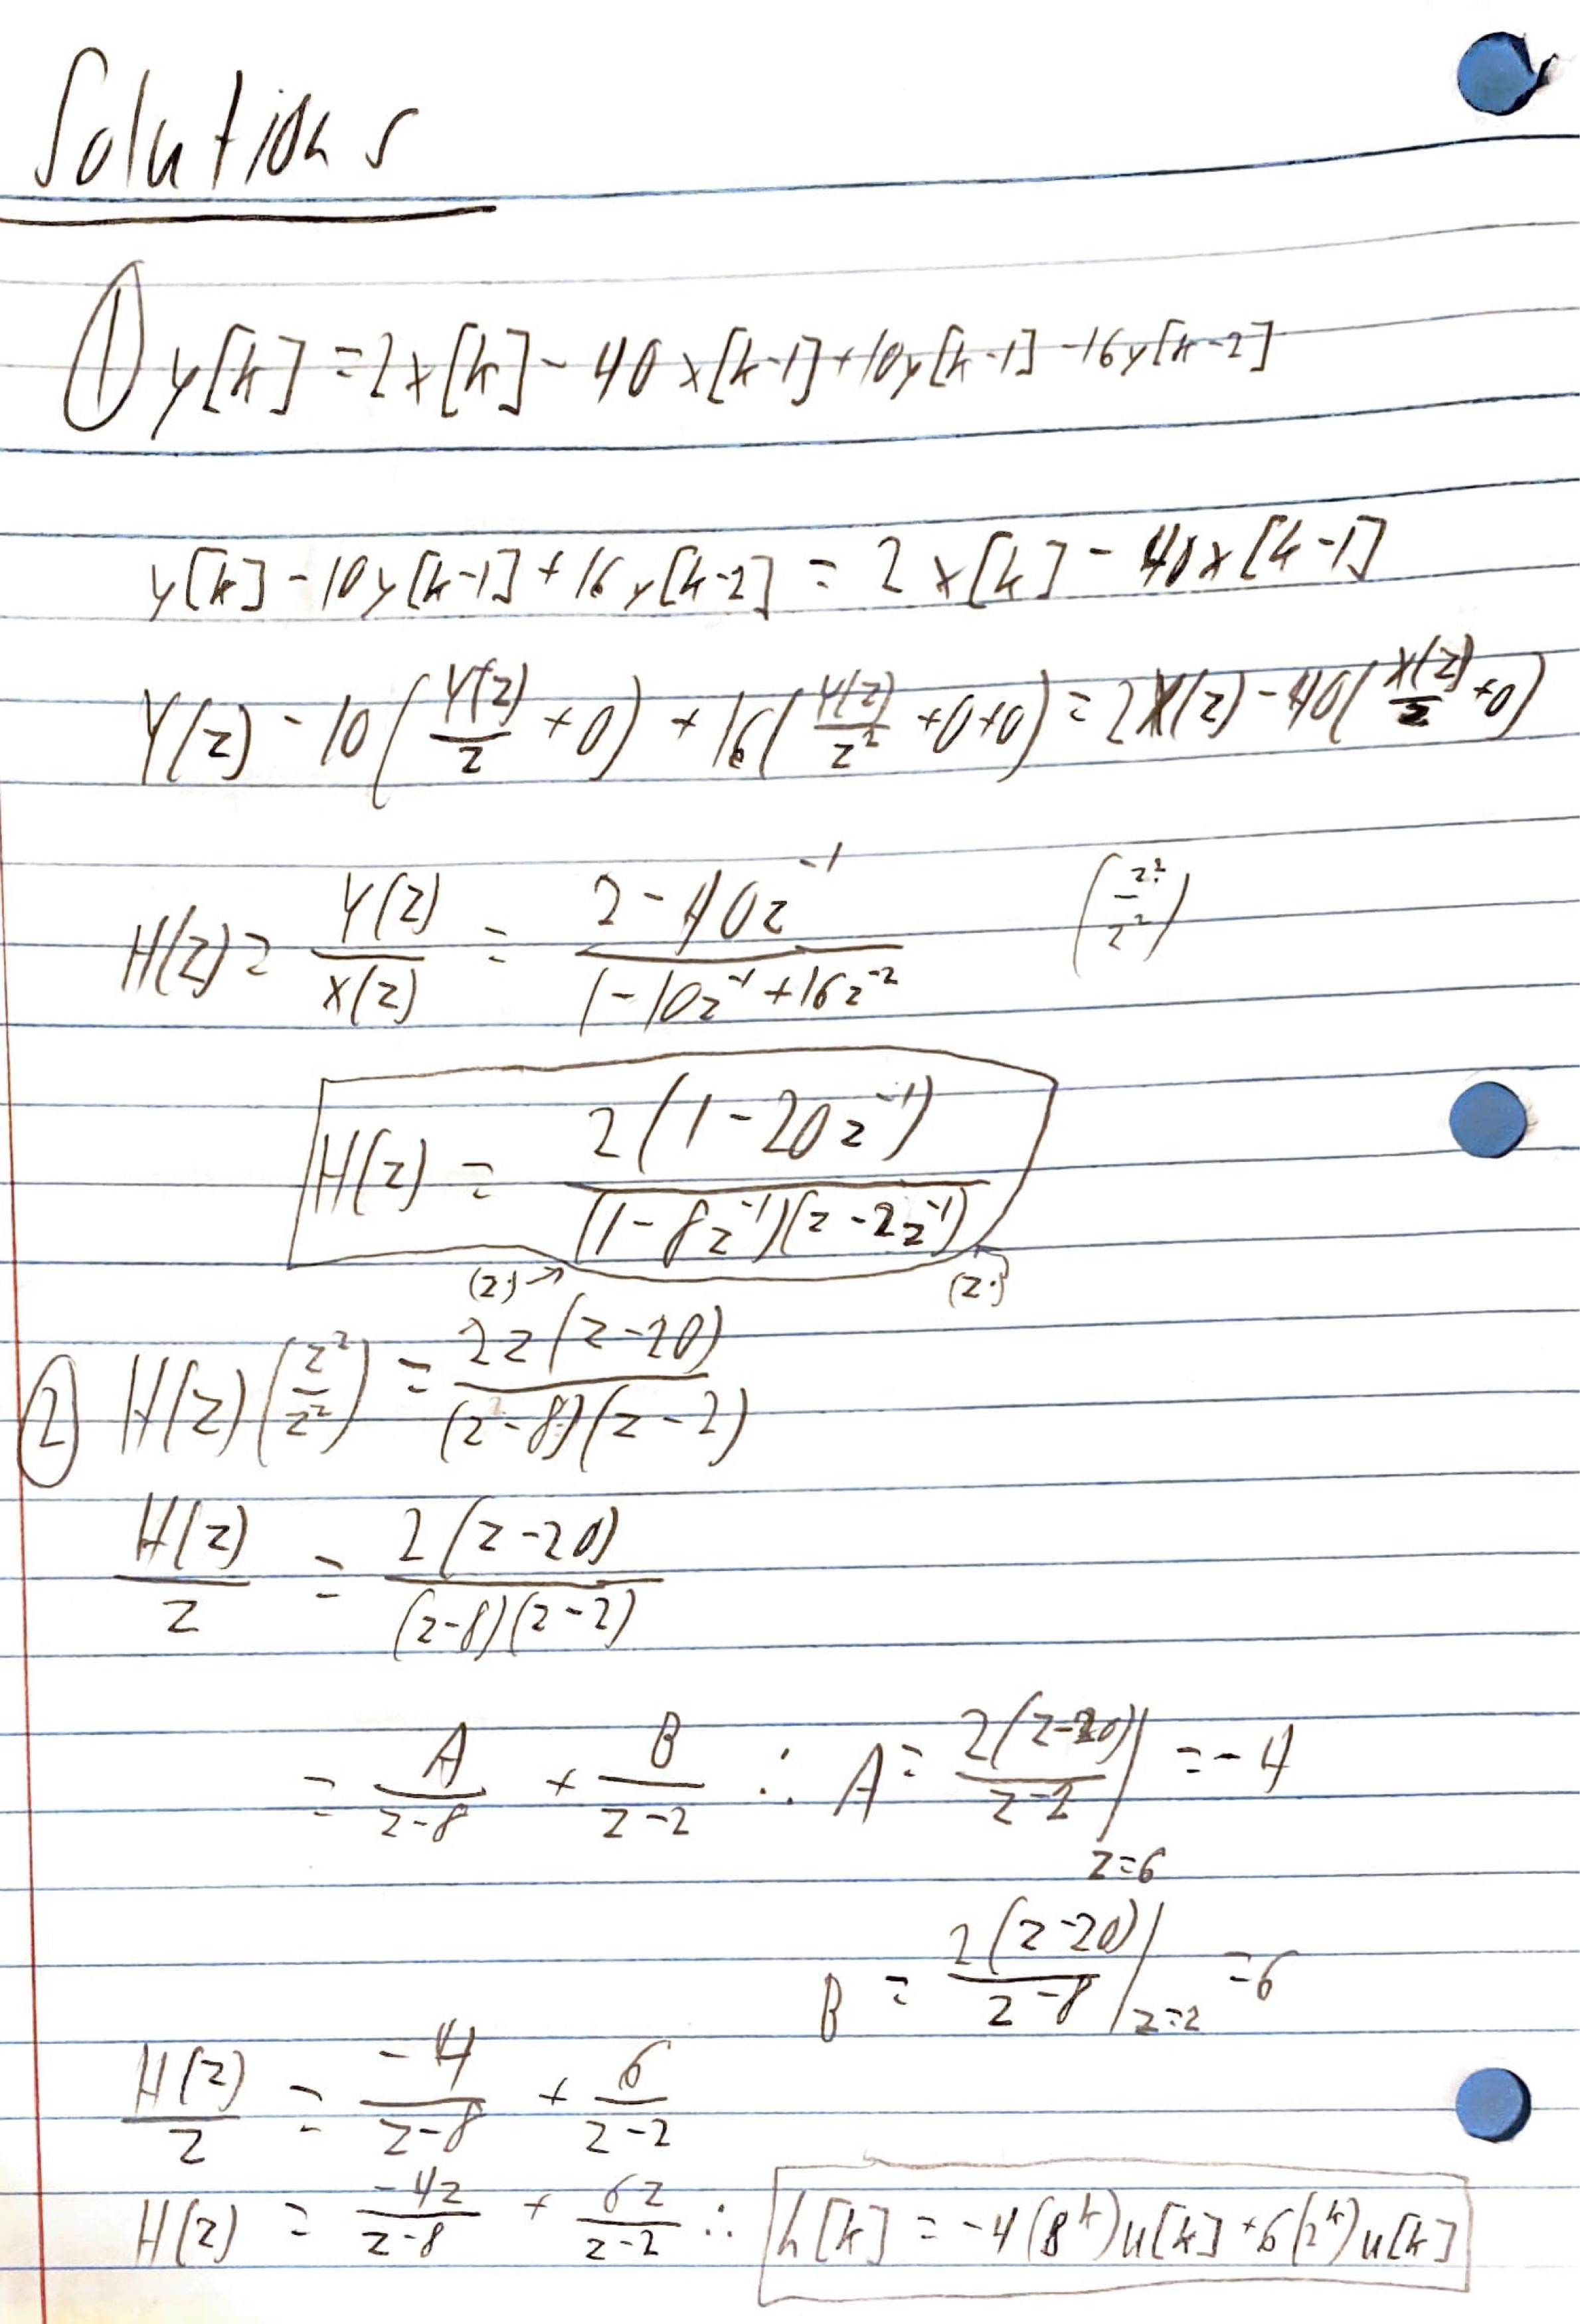
\includegraphics[scale=0.15]{FF23EEB3-DFB1-40FC-A79A-8F73C1F11979.jpeg}
    
    \paragraph{} There's a small typo in the above image. H(z)'s 2nd term should be $(1-2z^{-1})$. 
    
    \paragraph{} Above is H(z) and h[k] found by hand. Deriving h[k] required partial fraction expansion. In Spyder, I used scipy.signal.residuez() to verify the partial fraction expansion performed above. The results of the library function are in the appendix. 
    
    \paragraph{} I then brought the provided file containing the zplane() function into my Spyder project and imported it. Thankfully, the function auto-generated a pole-zero plot when I input H(z)'s numerator and denominator. 
    
    \paragraph{} Finally, I used scipy.signal.freqz() to plot the magnitude and phase responses of H(z). The function returned the frequency and a complex number. I had to convert the magnitude to dB and phase to degrees before plotting. Also, the plots looked best without a logarithmic scale, unlike bode plots.
    
\section{Results}

%This section will go over the results of the lab. Use this area to describe %if the lab worked as expected or if the results are unexpected or different %from your hand calculations or intuition. Part of being a good engineer is %gaining intuition about these problems and being able to understand quickly %if something is wrong. Use code, plots, tables, and figures as necessary. %Make sure to cite all other works used and note them in the bibliography. A %sample entry is in this document.
    
    \paragraph{} Initially, given the original function, I expected H(z) to hold a couple poles and a couple zeros. As seen previously, my expectation for the poles was correct since there's two poles, but there's also only a single zero at 20.
    
    \paragraph{} I didn't have many expectation for h[k] since lab 11 is the first time I've derived the z-transform of a function. So, it was hard to know what its inverse would be. I was unsurprised by the presence of step functions, but surely didn't predict the constants raised to the power of k. 
    
    \paragraph{} Taking the zplane of H(z), I expected to see the poles and zeros more readily in a graphical format. 
    
    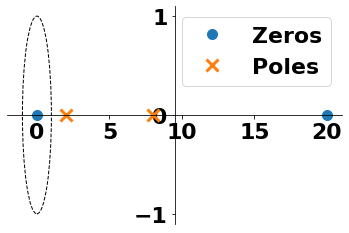
\includegraphics[]{Figure 2022-04-05 213446 (0).png}
    
    \paragraph{} As seen above, my expectation were spot on. I was surprised at how great the graphical representation truly turned out to be, with the legend provided. Although, I'm still somewhat confused about why there's a dashed oval around the zero at zero.
    
    \paragraph{} For the magnitude and phase, I expected the phase to go through a change of 180 degrees, since H(z) had two poles. I wasn't sure what to expect for the magnitude.
    
    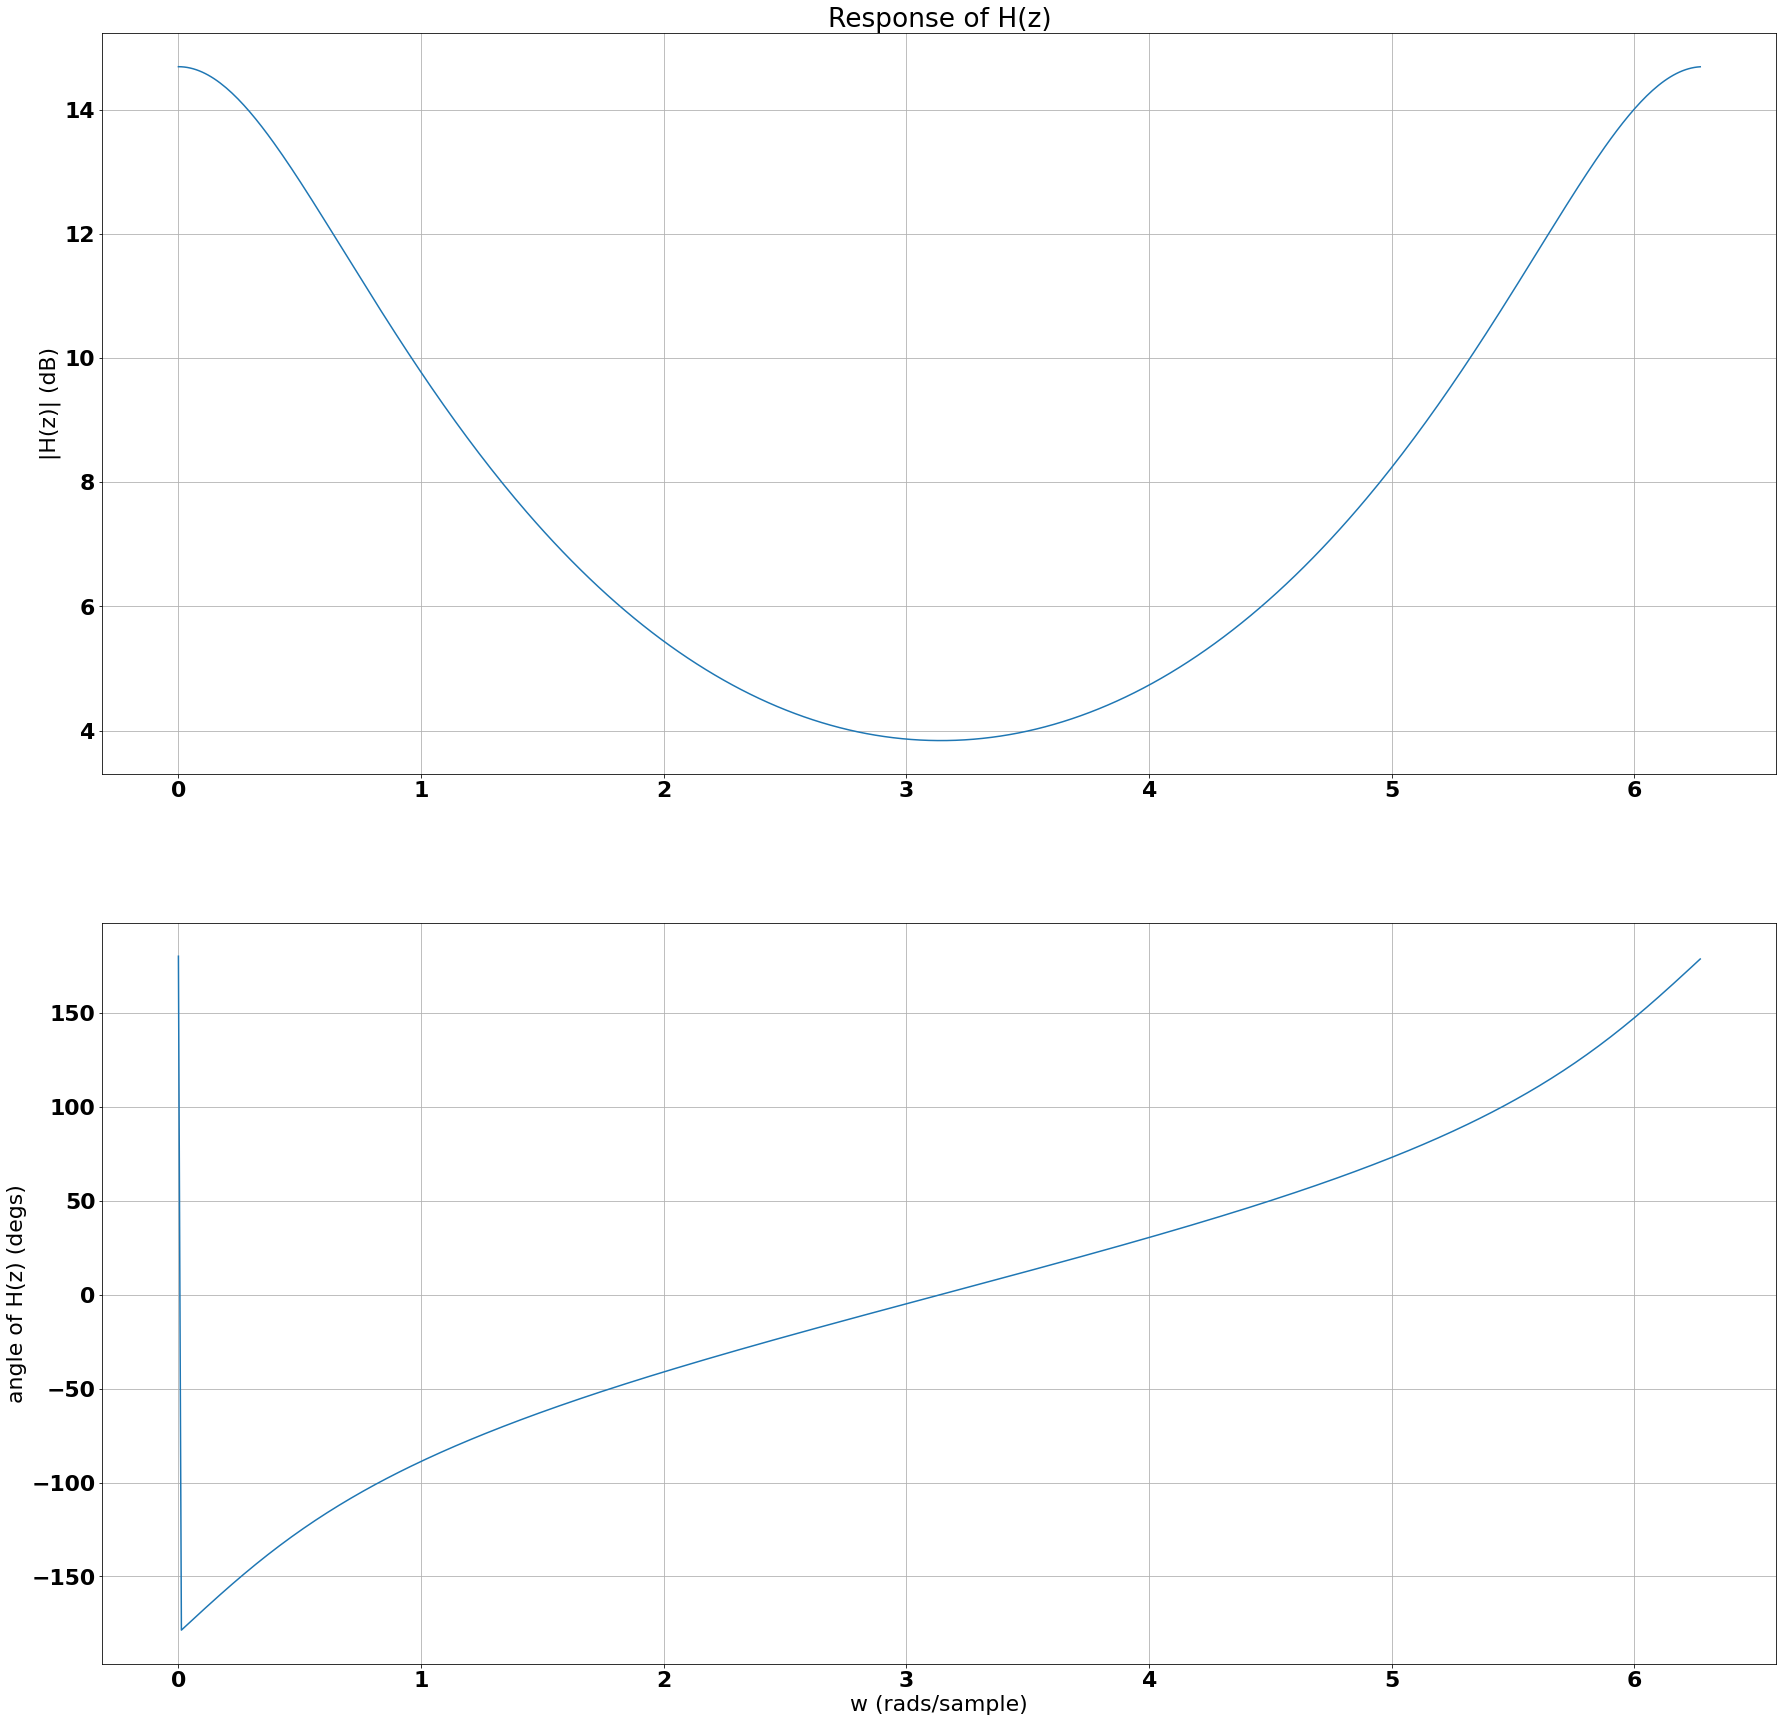
\includegraphics[scale=0.25]{Figure 2022-04-05 213446 (1).png}
    
    \paragraph{} As seen above, my expectation for phase was incorrect, since the function went through a 360 degree change. I was also surprised with how the magnitude never zeroed out, allowing all frequencies through with varying amounts of attenuation. This filter seems like a weak band-stop because of the u nature of the magnitude and how it never zeroes out. 

\section{Error Analysis}

%This section will discuss error analysis of the experiment. Since this lab %deals with ideal simulation there shouldn't be any sources of error, so %instead this section can be used to describe any difficulties you had during %lab and how you solved them. Alternatively, if you couldn't get the %experiment to work, which is okay, you need to use this section to explain why %you couldn't get it to work to earn full points. 

\paragraph{} The main difficulty I encountered was taking the z-transform of the original function. As previously mentioned, this lab was the first time I've done so. It took some learning from the book and help from the TA.

\paragraph{} A possible source of error is scipy.signal.freqz()'s approximation in computing the magnitude and phase. Also, my conversions for the magnitude into dB and phase into degrees. All of these contribute some small amount of approximation and therefore error.

\section{Questions} %also address any deliverables not yet put in yet
    \begin{enumerate}
        \item Looking at the plot generated in Task 4, is H(z) stable? Explain why or why not.
        \paragraph{} Yes, since all the poles are in the left half plane with respect to the graph constructed by the library function in Task 4. 
                
        \item Leave any feedback on the clarity of lab tasks, expectations, and deliverables.
        \paragraph{} The tasks of the lab, deliverables, and expectations were clear. 
    \end{enumerate}

\section{Conclusion}

%Discuss briefly what you learned in this lab and whether or not you feel the %lab was successful. Include any recommendations for future labs as this is a %learning experience for all of us. Discuss any insights you gained from this %lab and how that will affect future work. \textit{Note: The bibliograhpy %needs to be on its own page.}

    \paragraph{} During lab 11, I analyzed a discrete function for the first time using Python pre-built functions. I learned how to properly take the z-transform, and the appropriate method to use. Lab 11 was a success since I was able to find the z-transform by-hand and verify it using Python, which resulted in my better comprehension of z-transforms.
    
    Github: \url{https://github.com/SethCram} 

\appendix

\chapter{Library's Partial Fraction Expansion}
     Console output:
    \begin{lstlisting}
        partial fraction results:  [ 6. -4.]
        Corresponding poles:  [2. 8.]
        Coeffs of the direct polynomial terms:  []  
    \end{lstlisting}

\newpage

\end{document}